\section{Resultados}
\label{resultados}

\textbf{Estrutura e homofilia (H1).} $G_1$ tem 4.424 vértices, 49.532 arestas, grau médio 22{,}4, densidade 0{,}005, coeficiente de agrupamento 0{,}26 e uma única componente. Embora o desfecho não tenha sido usado na construção, 63{,}2\% das arestas ligam estudantes com o mesmo desfecho, contra 38{,}5\% esperados ao acaso, e a assortatividade é $r=0{,}39$. A Figura~\ref{fig-rede} mostra regiões nitidamente dominadas por evasão e por graduação. A matriz de mistura revela que os matriculados são os menos segregados: suas arestas se dividem entre graduados (7{,}5\% do total) e matriculados (5{,}2\%), o que é coerente com sua condição de desfecho ainda em aberto. Só com atributos de ingresso ($G_1^{\mathrm{ing}}$), a assortatividade cai para $0{,}18$, mas permanece positiva. \textbf{H1 é confirmada.}

\begin{figure*}[!ht]
\centering
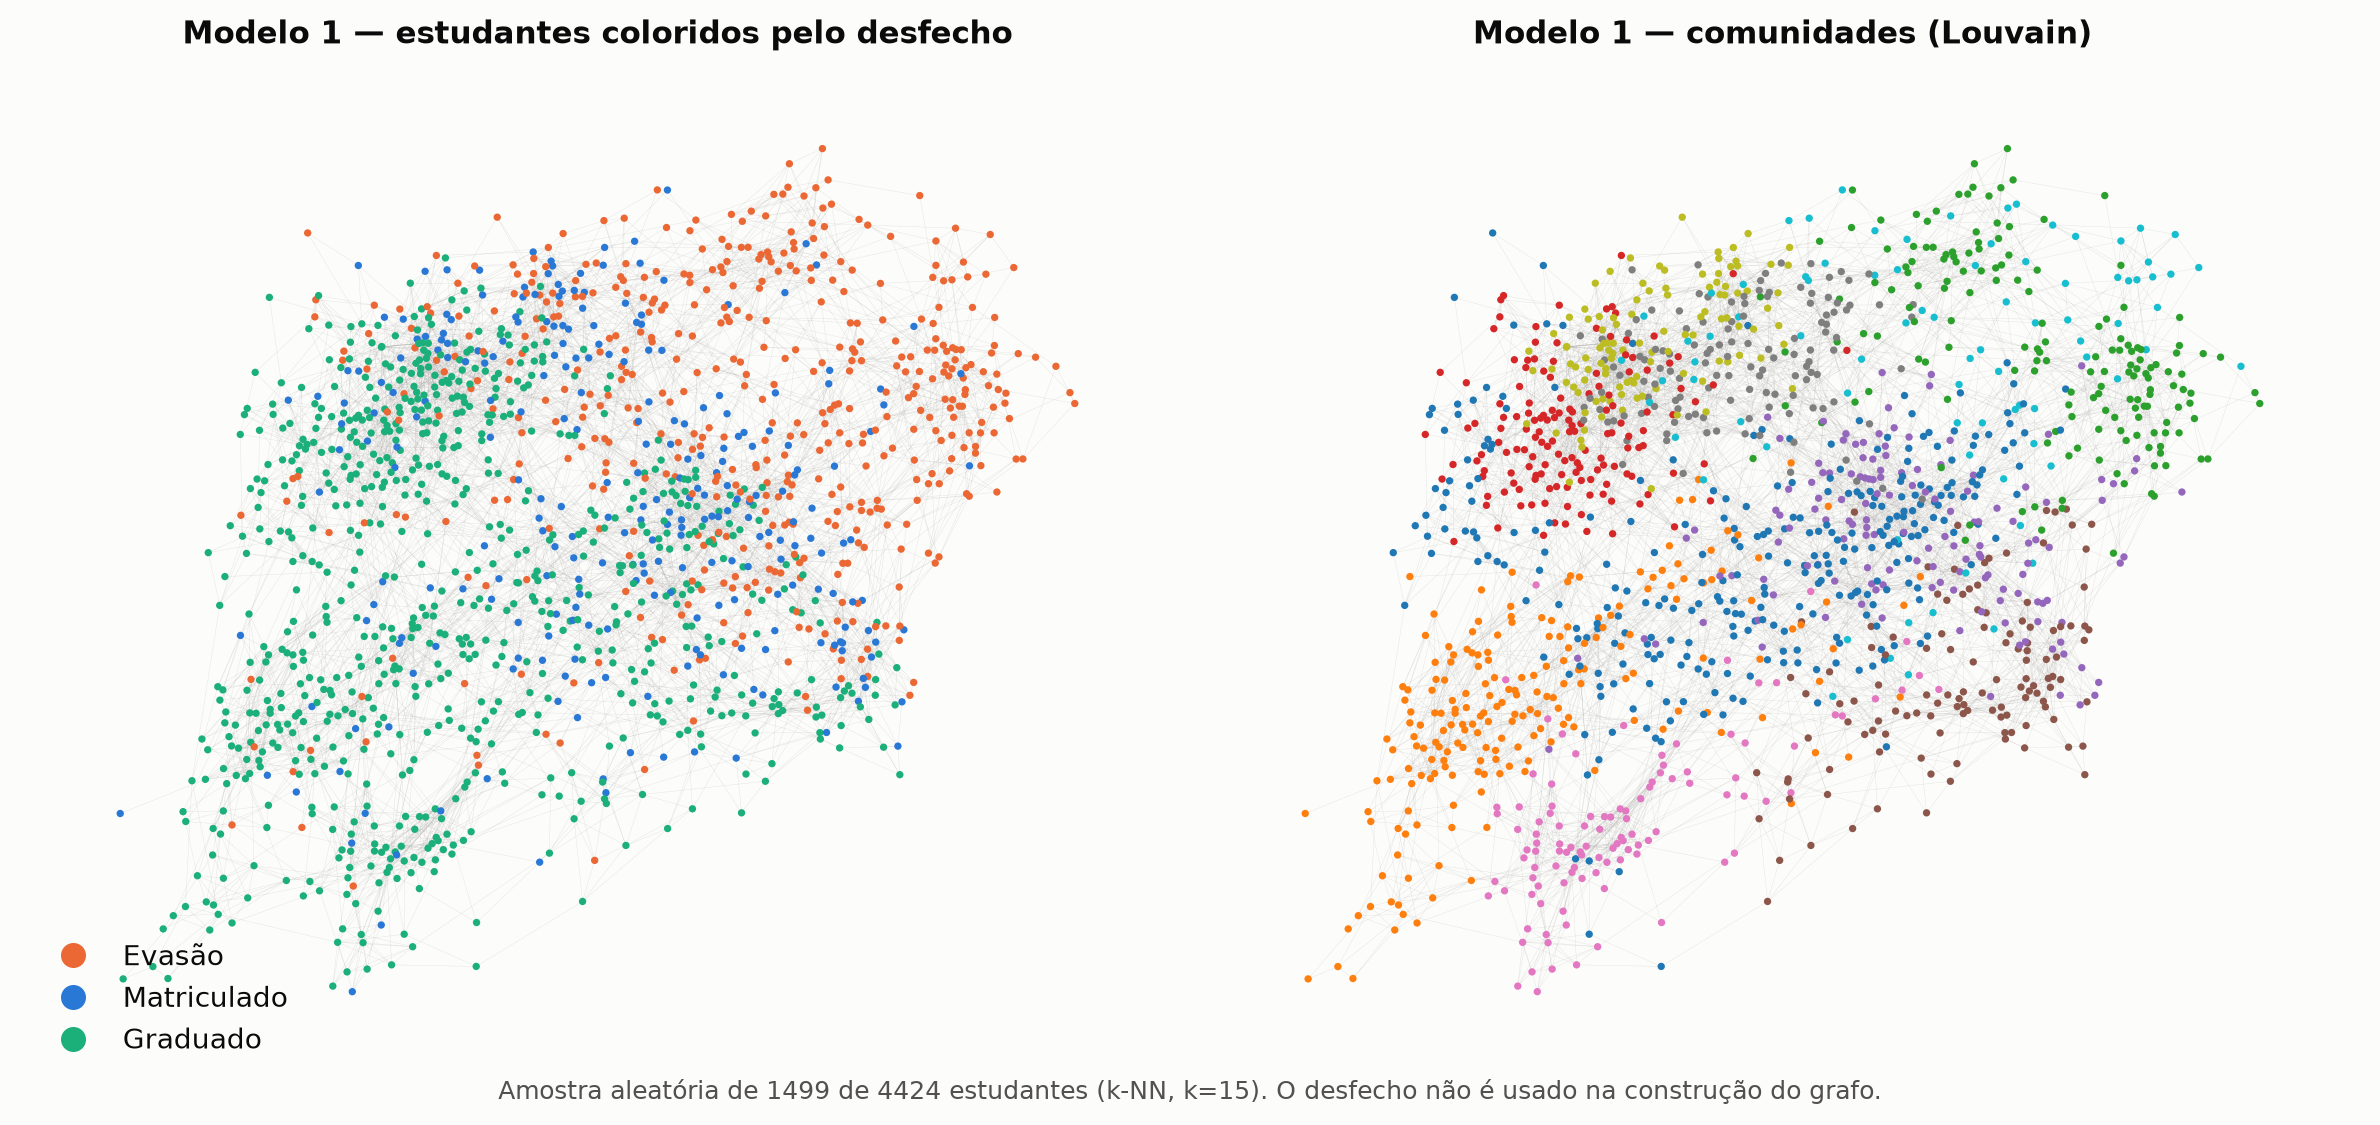
\includegraphics[width=0.92\textwidth]{figs/fig1_rede_similaridade.png}
\caption{Modelo 1 (rede de similaridade $k$-NN, $k=15$), amostra de 1.499 estudantes do dataset UCI~697: à esquerda, cor pelo desfecho; à direita, cor pela comunidade Louvain.}
\label{fig-rede}
\end{figure*}

\textbf{Comunidades e perfis (H2).} A Tabela~\ref{tab-comunidades} compara os métodos. O Louvain obteve a maior modularidade ($Q=0{,}715$, 12 comunidades), o Fast Greedy produziu menos comunidades e com menos arestas intercomunidades, e o Label Propagation fragmentou a rede. Assim como em \citet{porto2025}, o método altera bastante a granularidade da solução. NMI e ARI baixos são esperados, pois as comunidades representam \textit{perfis}, e não os desfechos. O que importa é a amplitude da taxa de evasão entre comunidades: 8\% a 94\% no Louvain (Figura~\ref{fig-comunidades}), contra a média institucional de 32\%.

\begin{table}[hbt!]
\caption{Comparação dos métodos de detecção de comunidades no Modelo 1.}
\label{tab-comunidades}
\resizebox{\columnwidth}{!}{
\begin{tabular}{|l|c|c|c|c|c|}
\hline
\rowcolor[HTML]{CBCEFB}
\textbf{Método} & \textbf{Com.} & $\mathbf{Q}$ & \textbf{\% inter} & \textbf{NMI} & \textbf{Amplit. evasão} \\ \hline
Louvain & 12 & \textbf{0,715} & 19,0 & \textbf{0,133} & 85,6 p.p. \\ \hline
Fast Greedy & 5 & 0,652 & \textbf{10,2} & 0,113 & 69,6 p.p. \\ \hline
Label Prop. & 70 & 0,603 & 37,4 & 0,123 & 93,7 p.p. \\ \hline
\end{tabular}}
\end{table}

\begin{figure}[!ht]
\centering
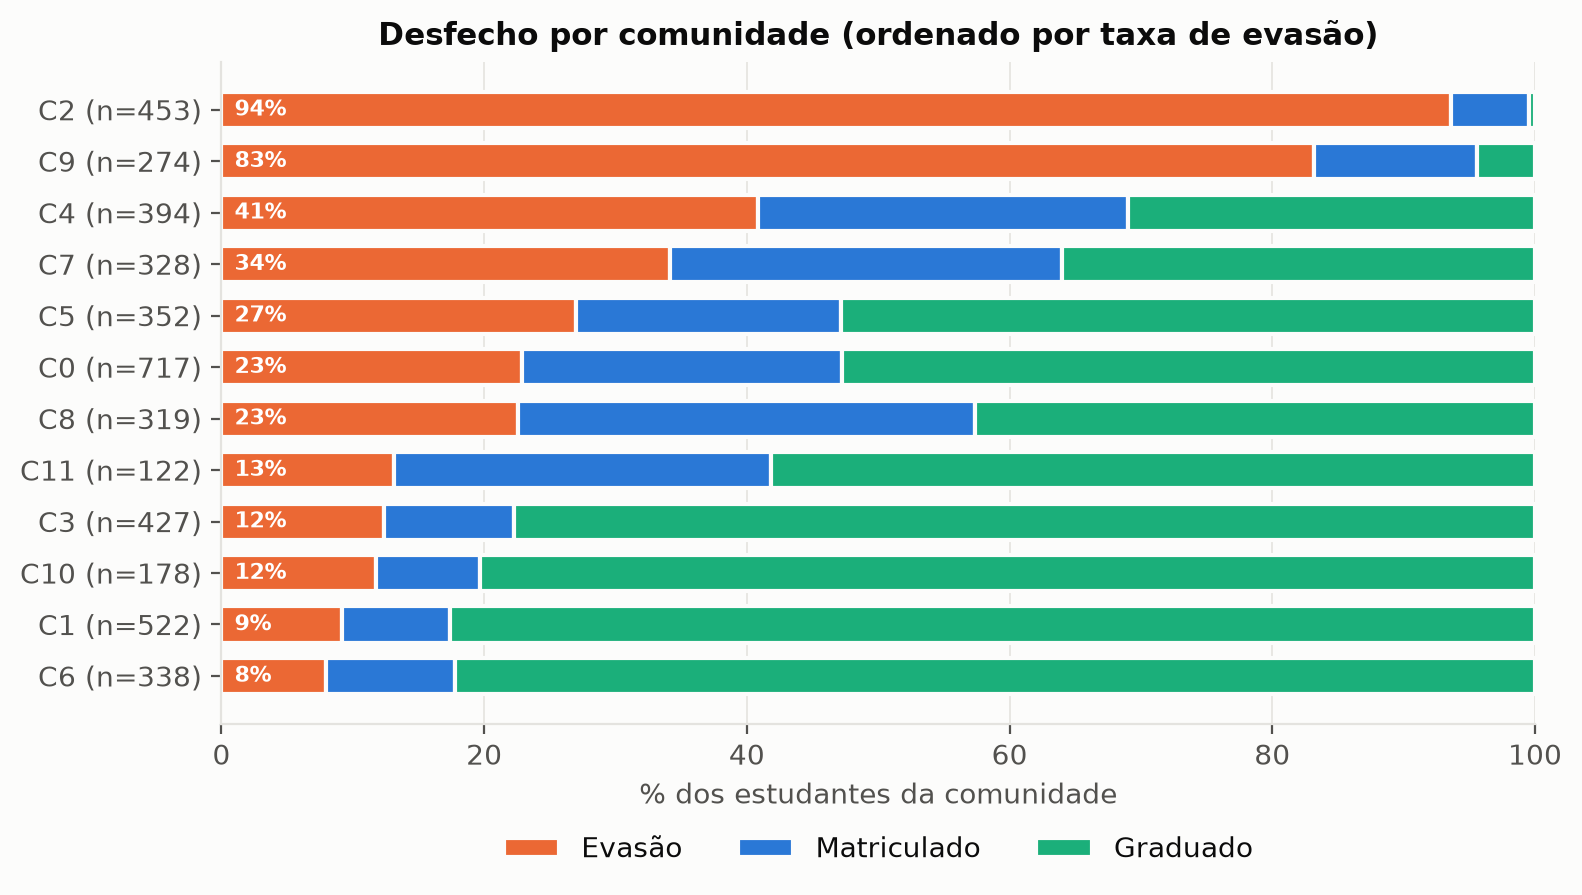
\includegraphics[width=0.48\textwidth]{figs/fig2_desfecho_por_comunidade.png}
\caption{Distribuição dos desfechos nas 12 comunidades Louvain do Modelo 1, ordenadas pela taxa de evasão.}
\label{fig-comunidades}
\end{figure}

Os fatores característicos tornam os grupos interpretáveis:
\textbf{C2} (453 estudantes, 94\% de evasão) reúne quem não aprovou nenhuma disciplina no 2º semestre (94\%), um padrão de \textit{abandono acadêmico};
\textbf{C9} (274, 83\%) é um perfil \textit{financeiro}, com 100\% de devedores e 85\% com mensalidade atrasada, embora a maioria tenha aprovação parcial;
\textbf{C4} (394, 41\%) concentra disciplinas sem avaliação, um sinal de desengajamento;
\textbf{C5} (352, 27\%) reúne adultos trabalhadores (30+, noturno, ``maiores de 23'') e evade \textit{menos} que a média, porque a maioria aprova tudo no 2º semestre. Embora a idade 30+ isolada esteja associada a 54\% de evasão, o grafo mostra que, dentro desse grupo, o desempenho é o que decide. Já \textbf{C1} e \textbf{C6} (bolsistas com aprovação plena, 8--9\%) são os perfis de \textit{sucesso}. \textbf{H2 é confirmada.}

\textbf{Perfis semelhantes, desfechos distintos.} Em $G_1^{\mathrm{ing}}$ há 2.382 pares Evasão$\times$Graduado com perfil de ingresso quase idêntico (similaridade $\geq 0{,}97$). Comparados a pares Graduado$\times$Graduado igualmente similares (Figura~\ref{fig-div}), o que os separa é a trajetória: a aprovação no 2º semestre difere em 79{,}5\% dos pares divergentes contra 45{,}3\% dos pares de controle (+34 p.p.), e a do 1º semestre em +25 p.p., seguidas do curso (+11 p.p.). Atributos socioeconômicos e demográficos praticamente não diferem. Além disso, 16{,}7\% dos evadidos têm $\leq 25\%$ de vizinhos evadidos em $G_1$, ou seja, são casos que um sistema baseado apenas em perfil não anteciparia.

\begin{figure}[!ht]
\centering
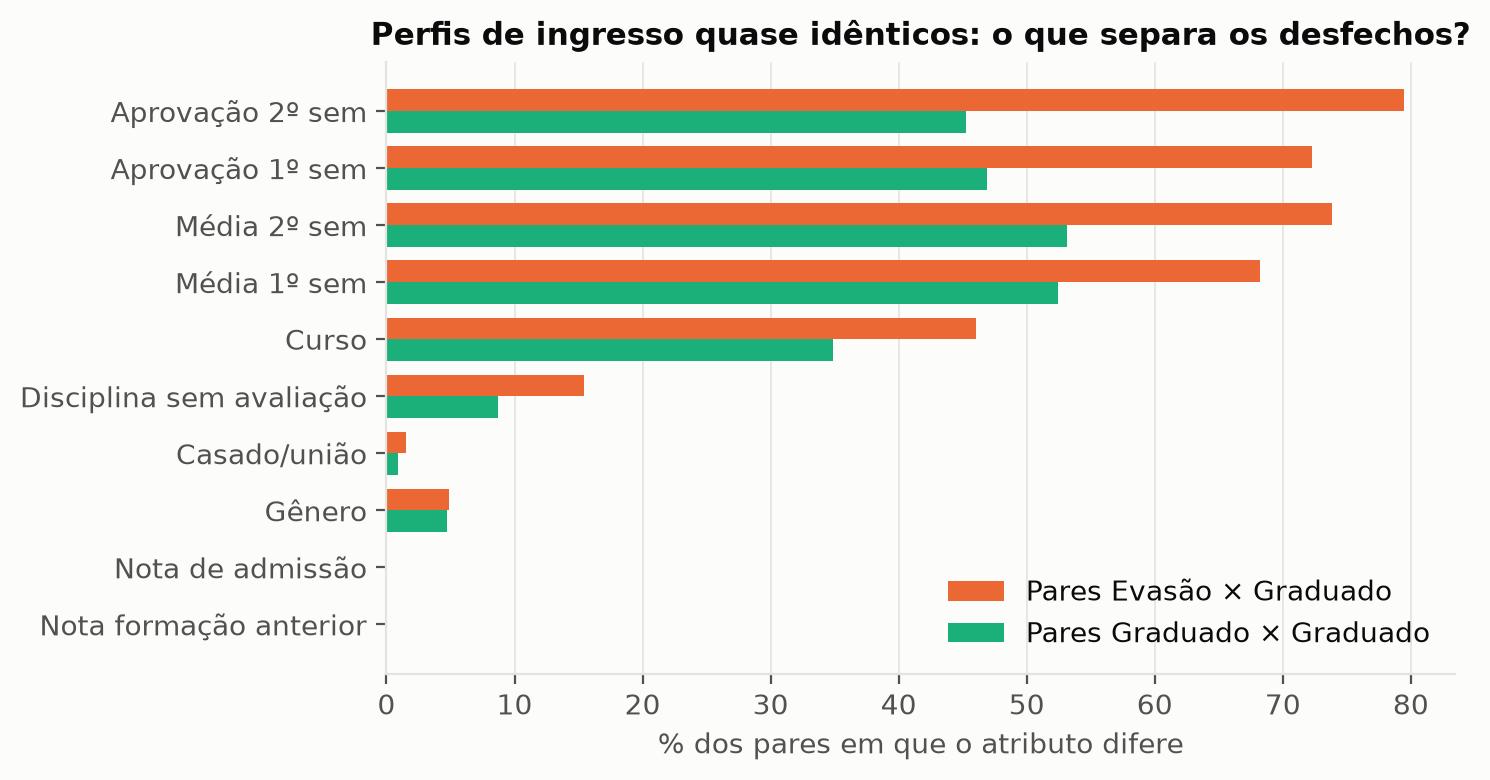
\includegraphics[width=0.48\textwidth]{figs/fig4_pares_divergentes.png}
\caption{Atributos que mais diferem em pares de estudantes com perfil de ingresso quase idêntico e desfechos opostos (Evasão$\times$Graduado) e em pares de controle.}
\label{fig-div}
\end{figure}

\textbf{Escore de risco relacional (H3).} Na Figura~\ref{fig-auc}, a propagação de rótulos no grafo atinge AUC $=0{,}899$, superior à do melhor atributo isolado (aprovação no 2º semestre, $0{,}856$) e próxima da regressão logística multivariada ($0{,}914$). Entre os 20\% de maior escore, 91{,}4\% de fato evadiram. Sem desempenho acadêmico, a vantagem sobre a variável isolada aumenta (0{,}774 contra 0{,}655 da idade). O híbrido acrescenta apenas +0{,}001 de AUC à logística: neste dataset, a vizinhança não traz informação preditiva além dos próprios atributos. Seu valor está na \textit{explicação} (``quem são os vizinhos e o que aconteceu com eles''). A análise de sensibilidade mostrou que o grafo só com ACAD é o mais modular ($Q=0{,}91$), mas tem AUC menor (0{,}866) do que a combinação multirrelacional (0{,}894). Grafos só com SOCIO ou só com DEMO ficam em 0{,}71--0{,}73. A combinação das dimensões é, portanto, o que melhor captura o desfecho. Variar $k$ entre 10 e 25 altera a AUC em menos de 0{,}01. \textbf{H3 é parcialmente confirmada}: o escore supera o indicador isolado, mas não o modelo tabular.

\begin{figure}[!ht]
\centering
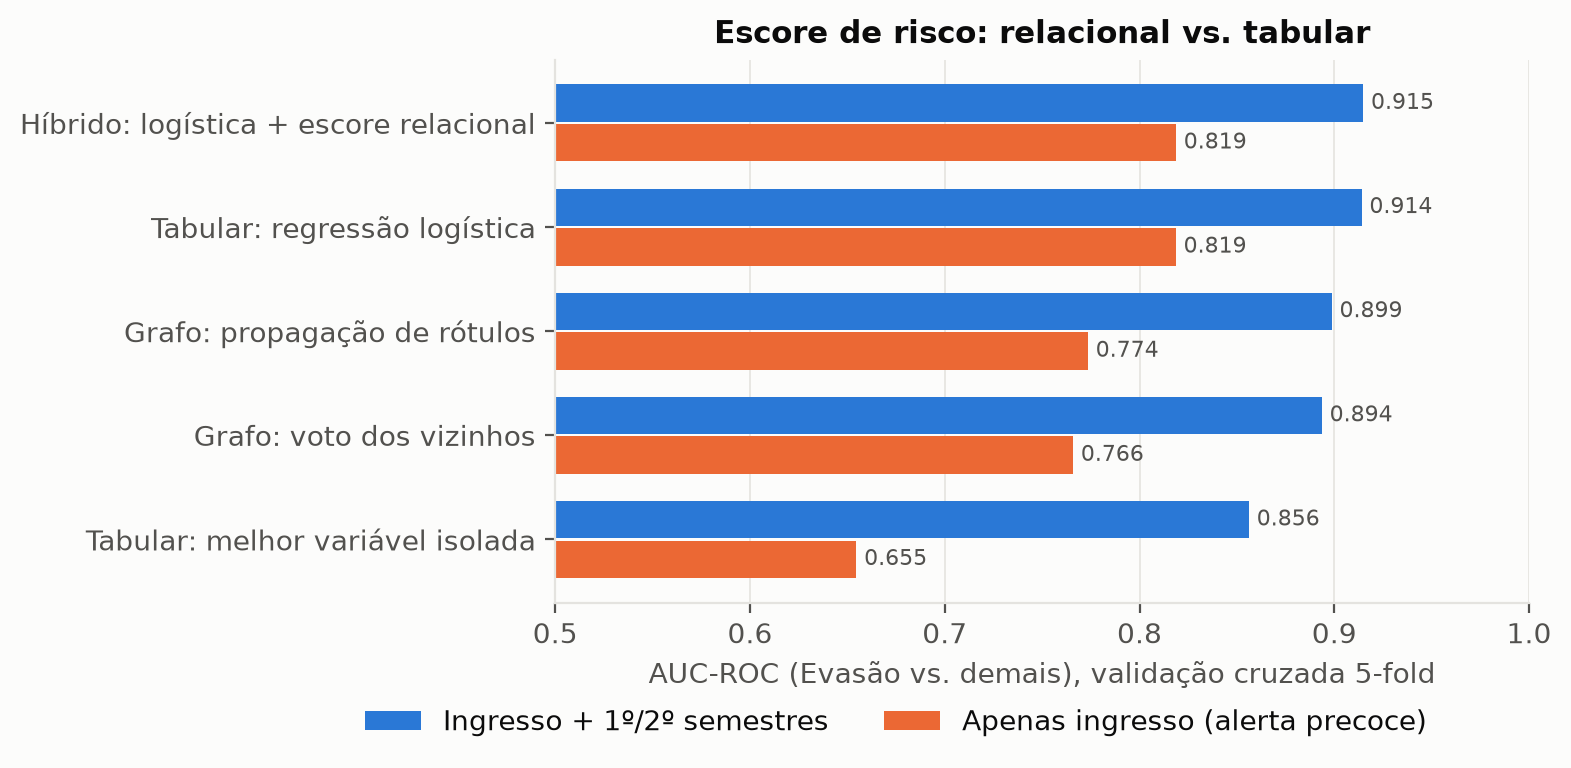
\includegraphics[width=0.48\textwidth]{figs/fig3_validacao_auc.png}
\caption{AUC-ROC (Evasão $\times$ demais) dos escores relacionais e tabulares em validação cruzada de 5 partições, com todos os atributos e somente com os de ingresso.}
\label{fig-auc}
\end{figure}

\textbf{Rede de fatores (H4).} $G_2$ tem 77 vértices e 513 arestas (densidade 0{,}18). O Louvain particiona os fatores em três comunidades principais, \textit{cada uma contendo exatamente um nó de desfecho} (Figura~\ref{fig-fatores}). O núcleo da \textbf{Evasão} (24 fatores) reúne aprovação nula ou baixa, inadimplência (mensalidade atrasada: lift 2{,}69; devedor: 1{,}93), ingresso ``maiores de 23'', idade 23+, turno noturno, casado(a), não bolsista e escolaridade fundamental dos pais. O do \textbf{Graduado} (32 fatores) reúne aprovação plena, médias $\geq 12$, bolsa, ingresso na 1ª fase, idade 17--19, deslocado e gênero feminino. O do \textbf{Matriculado} (12 fatores) reúne aprovação entre 50 e 99\%, médias $<12$, notas de admissão abaixo de 120, disciplinas sem avaliação e ingresso por transferência. A análise de sinergia mostra combinações que superam cada fator isolado: devedor (62\%) com ingresso ``maiores de 23'' (55\%) chega a 77\% de evasão; e aprovação parcial no 2º semestre (66\%) com idade 30+ (54\%) chega a 86\%. Os fatores de maior intermediação, como não bolsista, nota de admissão 140--160 e Gestão (noturno), funcionam como pontes entre os núcleos. \textbf{H4 é confirmada.}

\begin{figure*}[!ht]
\centering
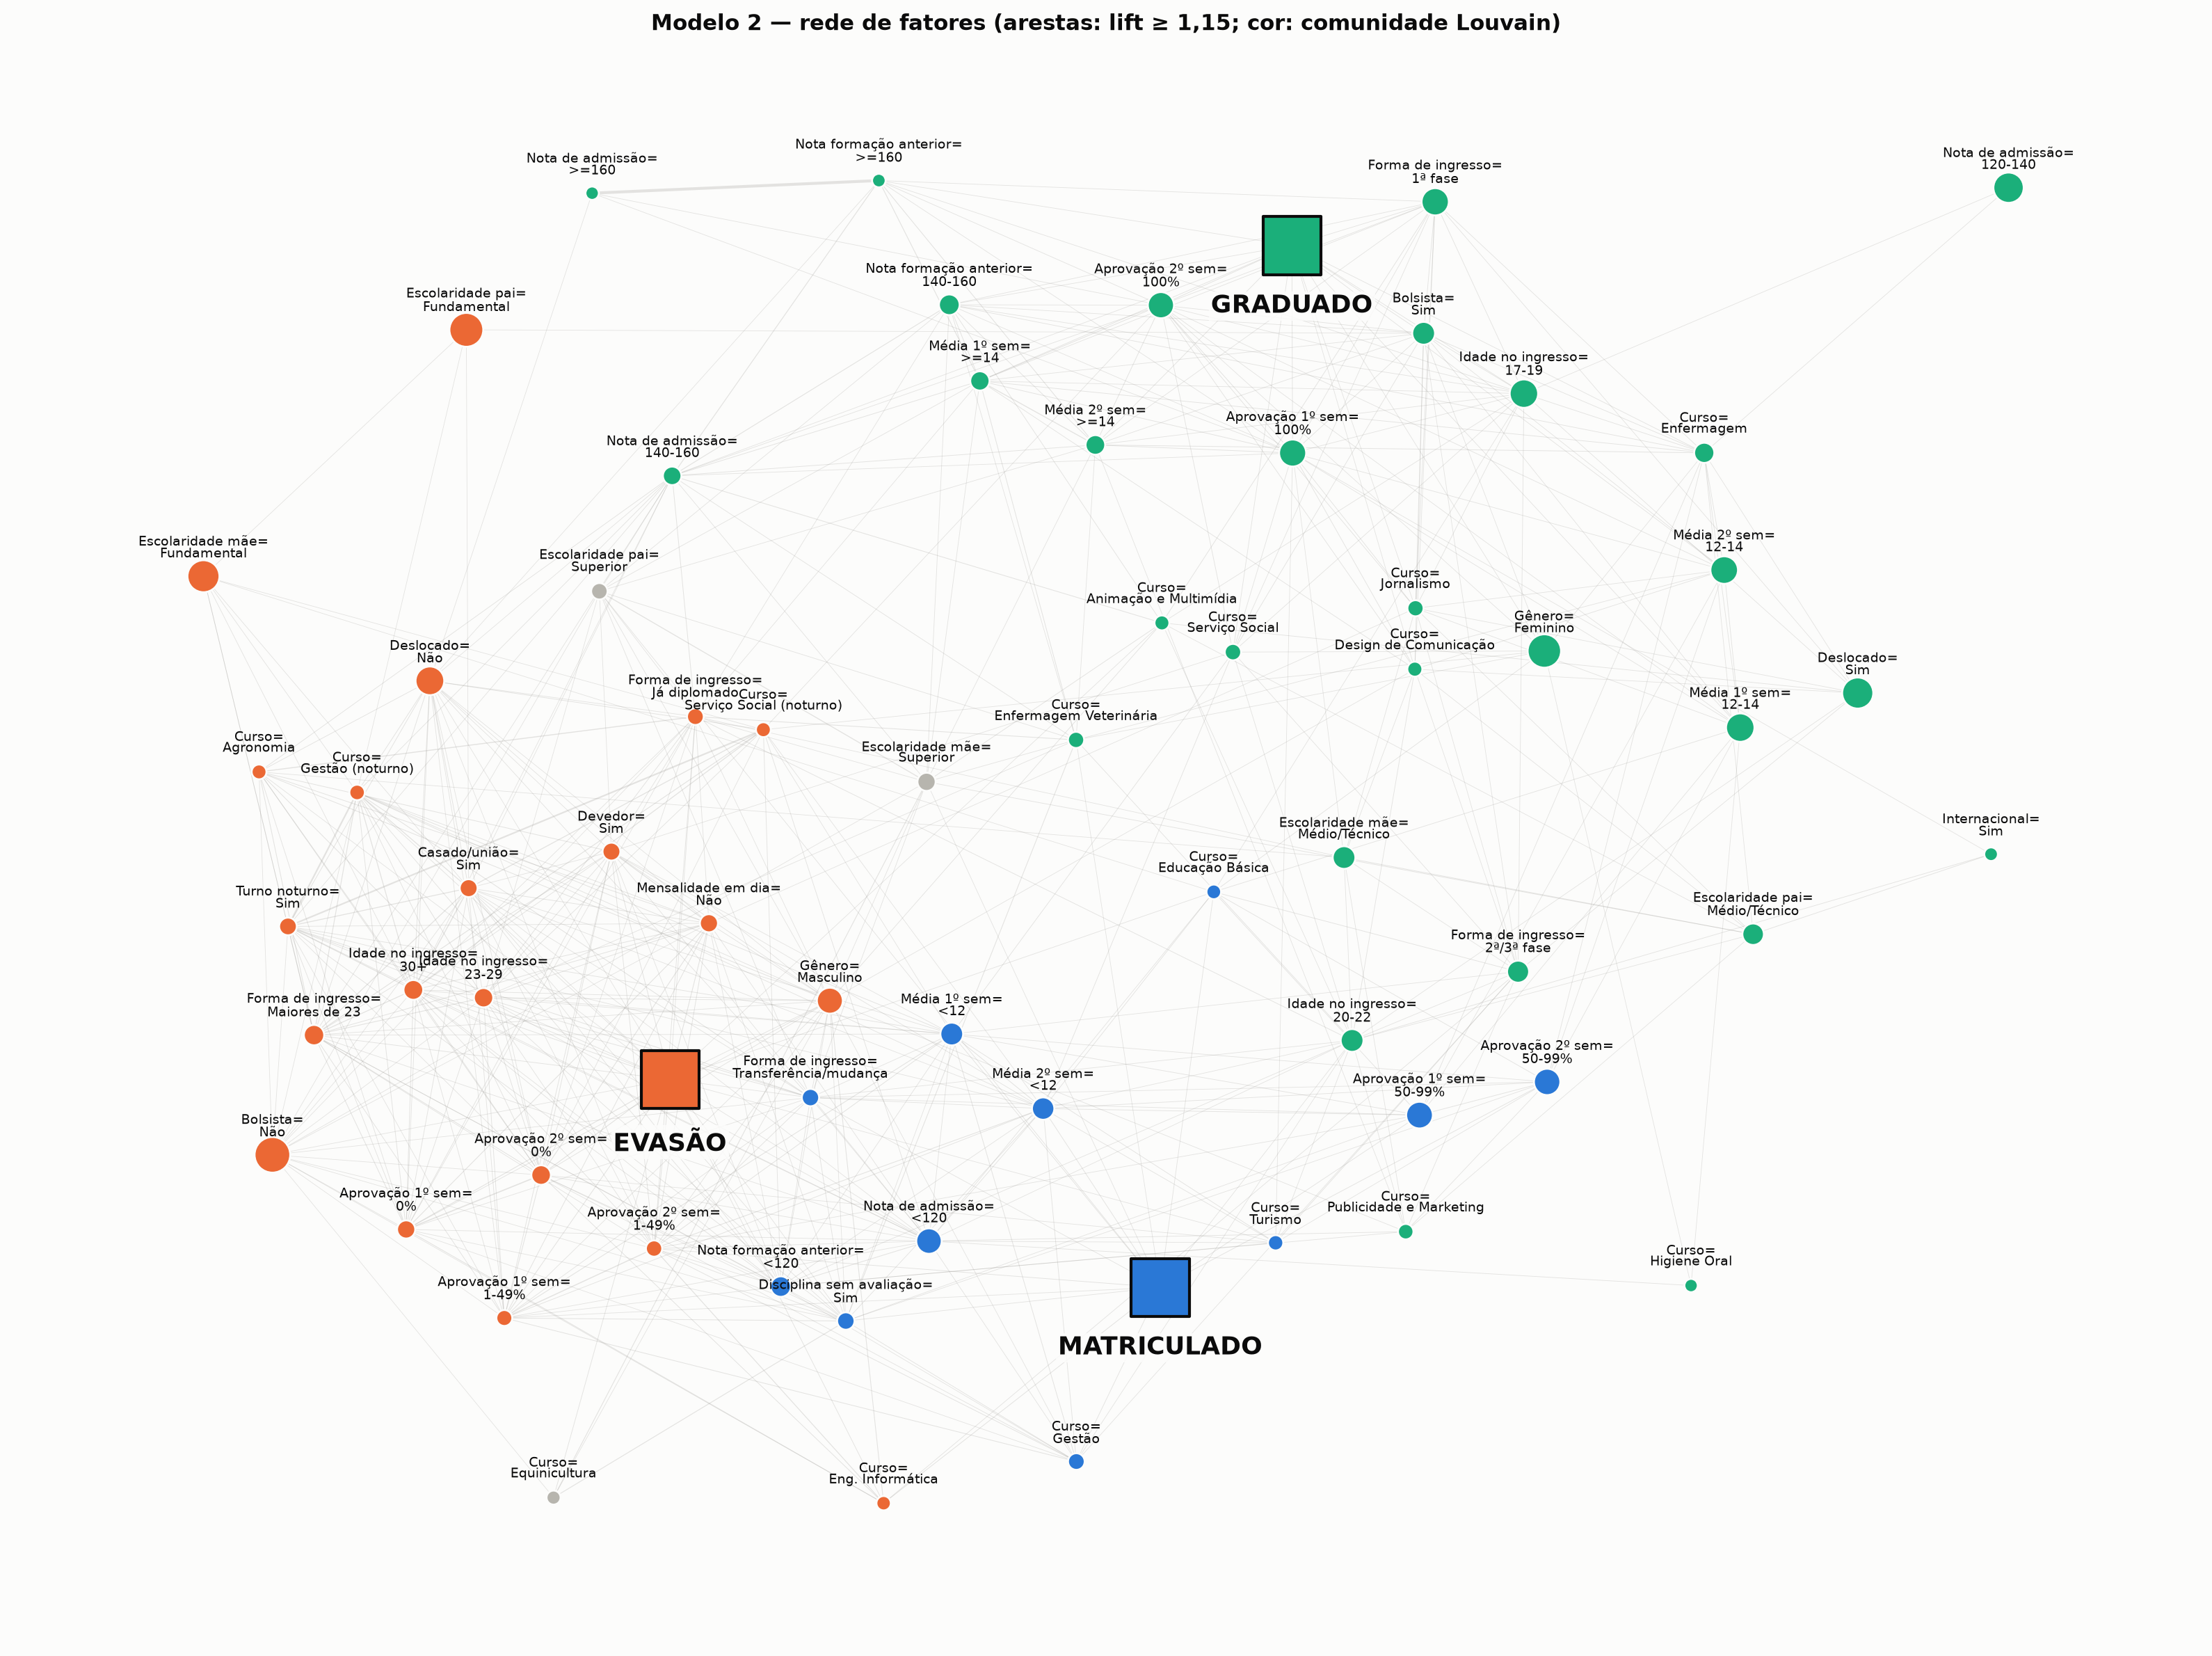
\includegraphics[width=0.85\textwidth]{figs/fig7_rede_fatores.png}
\caption{Modelo 2: rede de co-ocorrência de fatores (lift $\geq 1{,}15$) no dataset UCI~697, com nós quadrados de desfecho e cores das comunidades Louvain. Cada comunidade contém exatamente um desfecho.}
\label{fig-fatores}
\end{figure*}

\textbf{Discussão e limitações.} Os resultados confirmam a evasão como problema relacional: perfis e combinações de fatores explicam diferenças de desfecho que nenhum indicador isolado revela. Como aplicação institucional, as comunidades C2, C9 e C4 sugerem três frentes distintas: \textit{acompanhamento pedagógico} logo após o 1º semestre, \textit{apoio financeiro} e \textit{busca ativa} de quem deixou de ser avaliado. Para estudantes adultos e de turno noturno, o foco deve ser o desempenho, e não o perfil. As limitações são: dados de uma única instituição portuguesa, sem histórico de disciplinas ou semestres posteriores ao 2º; a classe ``matriculado'' tem desfecho incerto; a discretização e os pesos $\alpha,\beta,\gamma$ são escolhas de modelagem (mitigadas pela análise de sensibilidade); e associações de lift não são causais.
